\documentclass{beamer}
% Option [handout] in der Beamer-Klasse fuehrt dazu, dass alles gleich 
% aufgedeckt ist. Nuetzlich, falls die Folien verschickt oder gedruckt 
% werden sollten

%----TITEL----------------------------------------------------------%
\author[Barthel, Funke, Richter]{R. Barthel, G. Funke, N. Richter}
\title[Finite Differenzen Methode f\"ur die Schr\"odinger Gleichung]{Finite Differenzen Methode f\"ur\\ die Schr\"odinger Gleichung}
\institute[Numerik-Praktikum 24/25]{Numerisches Praktikum\\
                    WS 2024/2025\\
                      Universit\"at Leipzig}
\date[WS 2025]{3.\ Februar 2025}


%-------------------------------------------------------------------%


%-----OPTIONEN BEAMER-----------------------------------------------%
\usetheme{default}

\setbeamertemplate{headline}{}
\setbeamertemplate{footline}{%
         \phantom{x}\hspace{5pt} \insertshortauthor  
         \qquad\qquad \insertshorttitle 
         \qquad\qquad\qquad \insertshortdate 
         \hfill S.\,\insertframenumber\phantom{xy}\vskip3pt}
\usefonttheme[onlymath]{serif}
%-------------------------------------------------------------------%

\usepackage{amsmath,amsthm,amsfonts,amssymb,graphicx,animate}

\usepackage[ngerman]{babel}
%\usepackage[utf8x]{inputenc}  % in alten Latex-Versionen fuer die Eingabe z.B. 
                               % von Umlauten

\usepackage{pgfplots}
\pgfplotsset{compat=1.18}
\usepackage{tikz}
\usetikzlibrary{arrows,shapes,positioning}

\usepackage{listings}
\lstset{basicstyle=\scriptsize\ttfamily,frame=lines,breaklines=true}





%----------------------- Macros and Definitions --------------------------

 \definecolor{mycyan}{rgb}{0.0, 1.0, 1.0}

% hier koennen Befehle definiert werden
\newcommand{\Div}{\operatorname{div}}


\begin{document}



%%%%%%%% Titlepage%%%%%%%%%%%%%%%%%%%%%%%%%%%%%%%%%%
\frame{\titlepage}
%%%%%%% Introductory slides%%%%%%%%%%%%%%%%%%%%%%%%%

\begin{frame}
\frametitle{Inhalt}
\tableofcontents
\end{frame}

\section{Aufgabenstellung}

\begin{frame}
    \frametitle{Schrödinger Gleichung}

    Die Schrödinger Gleichung auf $\mathbb{R}$ ist gegeben durch
    \begin{align*}
        iu_t - u'' + \lambda |u|^2u &= 0 \\
        u(x,0) &= \phi(x)
    \end{align*}
    
    mit $u:\mathbb{R}\times\mathbb{R}\to\mathbb{C}$, $\phi:\mathbb{R}\to\mathbb{C}$ und $\lambda\in\mathbb{R}$\\
    \ \\
    Im Folgenden gilt:
    \begin{itemize}
        \item $\lambda = -2$
        \item $u(x,t)=\frac{3}{2}\exp(i(\frac{5}{4}t-x))\text{sech}(\frac{3}{2}(x+5)-3t)$
        \item $\phi(x)=u(x,0)$
    \end{itemize}
\end{frame}

\begin{frame}
    \frametitle{Aufgaben}
    \begin{itemize}
        \item Implizites Finite Differenzen Verfahren für verschiedene $\epsilon$ implementieren
        \item Erhaltungsgrößen auswerten
        \item Explizites Finite Differenzen Verfahren mit implizitem Verfahren vergleichen
    \end{itemize}
    
\end{frame}

\section{Implizite Lösung}

%Herleitung für Diskretisierung?

\begin{frame}
    \frametitle{Herleitung}

    Zeitzentrierte implizite Diskretisierung {\small(Crank-Nicolson)}:

    Sein $\Delta t, \Delta x>0$.
    Approximiere $\partial_t u = \partial_x^2 u - \lambda |u|^2u$ zur Zeit $\Delta t (k+\frac{1}{2})$ im Ort $\Delta x j$ durch
    \begin{align*}
        \frac{U^{k+1}_j-U^{k}_j}{\Delta t} &= \frac{1}{2}(\frac{U^{k}_{j+1}-2U^{k}_j+U^{k}_{j-1}}{\Delta x}+\frac{U^{k+1}_{j+1}-2U^{k+1}_j+U^{k+1}_{j-1}}{\Delta x})\\
        &\quad\qquad -\frac{\lambda}{2}(|U^{k+1}_j|^2U^{k+1}_j+|U^{k}_j|^2U^{k}_j)
    \end{align*}
    Dabei ist
    \begin{align*}
        \frac{\lambda}{2}(|U^{k+1}_j|^2U^{k+1}_j+|U^{k}_j|^2U^{k}_j) \approx \frac{\lambda}{4}(|U^{k+1}_j|^2+|U_j^k|^2)(U^{k+1}_j+U_j^k)
    \end{align*}
    

\end{frame}

\begin{frame}
    \frametitle{Herleitung}

    Zusammenfassen der Ortskomponenten und umschreiben mit 
    \begin{align*}
        A = \begin{bmatrix}
            2  & -1 &  0  &  \cdots  & 0 \\
            -1  & 2 &  -1  &  \cdots  & 0 \\
            0  & -1 &  2  &  \ddots  & 0 \\
            \vdots & \vdots & \ddots & \ddots & -1 \\
            0 & 0 & 0 & -1 & 2\\
        \end{bmatrix}
    \end{align*}
    liefert
    \begin{align*}
        i\frac{1}{\Delta t}(U^{k+1}-U^k)&+\frac{1}{2|\Delta x|^2}(AU^{k+1}+AU^k)+F_k(U^{k+1})=0\\
        (F_k(U))_j &= \frac{\lambda}{4}(|U_j|^2+|U_j^k|^2)(U_j+U_j^k)
    \end{align*}
    Dies kann umgeschrieben werden zu
    \begin{align*}
        U^{k+1} = (\frac{i}{\Delta t}I + \frac{A}{2\Delta x^2})^{-1}((\frac{i}{\Delta t}I - \frac{A}{2\Delta x^2})U^k - F_k(U^{k+1}))
    \end{align*}

\end{frame}

\begin{frame}
    \frametitle{Diskretisierung}

    Sein $\Delta t, \Delta x>0$ mit $J=\frac{30}{\Delta x},K=\frac{6}{\Delta t}\in\mathbb{N}$.\\
    Approximiere $u(j\Delta x, k\Delta t)$ durch $U_j^k$ f\"ur $j=-J, .. , J,\ k=0, .. , K$\\
    \ \\
    Startbedingung: $U_j^0=\phi(j\Delta x)\ \forall j\in\{-J, -J+1, .., J\}$\\
    %Randbedingung: $U_{-J}^k=U_{J}^k=0\ \forall k\in\{0, .., K\}$\\
    % Randbedingungen sind nicht gegeben
    Fixpunktiteration:
    \begin{align*}
        U_p = (\frac{i}{\Delta t}I + \frac{A}{2\Delta x^2})^{-1}((\frac{i}{\Delta t}I - \frac{A}{2\Delta x^2})U^k - F_k(U_p))
    \end{align*}
    mit $| U_{i+1}-U_{i} |<\epsilon$ als Abbruchskriterium und
    \begin{align*}
        (F_k(U))_j = \frac{\lambda}{4}(|U_j|^2+|U_j^k|^2)(U_j+U_j^k)
    \end{align*}
\end{frame}

\begin{frame}
    \frametitle{Eine Lösung}

    %Insert NLS_abs.gif here

\end{frame}

\begin{frame}
    \frametitle{Das Phasenproblem}

    %NLS_real.gif und NLS_imag.gif

\end{frame}

\section{Energieerhaltung}

\begin{frame}
    \frametitle{Energie}

    Erhaltungsgrößen von Lösungen der PDG
    \begin{align*}
        \int_\mathbb{R} |u|^2 dx &= \text{const}\\
        \int_\mathbb{R} \frac{1}{2}|u'|^2 + \frac{\lambda}{4}|u|^4 dx &= \text{const}
    \end{align*}
    \ \\
    Diskretisierte Energien
    \begin{align*}
        \Delta x \sum_{j=-J}^J |U_j^k|^2 &= \Delta x \sum_{j=-J}^J |U_j^0|^2\\
        \frac{\Delta x}{2} \sum_{j=-J}^{J-1} |\frac{U_{j+1}^k-U_j^k}{\Delta x}|^2+\frac{\lambda}{4}\Delta x \sum_{j=-J}^J |U_j^k|^4 &= \text{const}
    \end{align*}

\end{frame}

\begin{frame}
    \frametitle{Energieverlust}

    \begin{figure}
        \begin{center}
            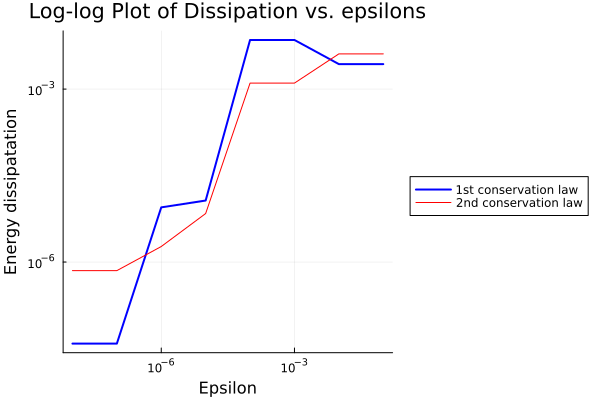
\includegraphics[width=0.7\textwidth]{../plots/eps-diss.png}
        \end{center}
    \end{figure}

\end{frame}

\section{Explizite Lösung}

\begin{frame}
    \frametitle{Explizietes Verfahren}

    Diskretisierung ohne Trapezregel liefert explizites Verfahren

    \begin{align*}
        \frac{i}{\Delta t} (U^{k+1}-U^k)-\frac{1}{|\Delta x|^2}AU^k+F_k(U^k)=0
    \end{align*}
    mit $F_k(U)$ wie zuvor. Also
    \begin{align*}
        U^{k+1}=U^k+\frac{\Delta t}{i|\Delta x|^2}AU^k-\frac{\Delta t}{i}F_k(U^k)
    \end{align*}

    % Gif einfügen

\end{frame}

\begin{frame}
    \frametitle{Instabilität}

    Explizites Verfahren stark Instabil
    \begin{itemize}
        \item $T = 0.4$
        \item $dt = 10^{-7}$
        \item $dx = 10^{-2}$
    \end{itemize}
    \ \\
    Divergiert ab ca. $t=0.6$

    % GIFs einfügen

\end{frame}

\end{document}
